\documentclass[conference]{IEEEtran}
\IEEEoverridecommandlockouts
% The preceding line is only needed to identify funding in the first footnote. If that is unneeded, please comment it out.
\usepackage{cite}
\usepackage{amsmath,amssymb,amsfonts}
\usepackage{algorithmic}
\usepackage{graphicx}
\usepackage{textcomp}
\usepackage{xcolor}
\usepackage{float}
\usepackage{subfig}
\usepackage{booktabs}
\usepackage{tabularx,booktabs,array} % in preamble
\usepackage{url}

\usepackage{tikz}
\usetikzlibrary{shapes,arrows,positioning}

\tikzset{
    base/.style={draw, text centered, font=\tiny, inner sep=2pt},
    block/.style={base, rectangle, fill=blue!5, text width=2.1cm, rounded corners, minimum height=0.6cm},
    cloud/.style={base, ellipse, fill=red!5, text width=2cm},
    decision/.style={base, diamond, fill=green!5, text width=1.2cm, aspect=2},
    model/.style={base, rectangle, fill=orange!10, text width=2.2cm, thick, minimum height=0.6cm},
    line/.style={draw, -latex, thin}
}
\def\BibTeX{{\rm B\kern-.05em{\sc i\kern-.025em b}\kern-.08em
    T\kern-.1667em\lower.7ex\hbox{E}\kern-.125emX}}

\begin{document}




\title{EfficientNet-GCN: A Hybrid Framework for
Explainable Osteoporosis Severity Classification in Multi-Class Knee Osteoporosis X-ray Images}
\author{
\IEEEauthorblockN{1\textsuperscript{st}Tasnim Sultana Sintheia}
\IEEEauthorblockA{\textit{Computer Science and Engineering} \\
\textit{American International University-Bangladesh (AIUB)}\\
Dhaka, Bangladesh \\
26-93981-1@student.aiub.edu}
\and
\IEEEauthorblockN{2\textsuperscript{th}Musfique Rahman Muin}
\IEEEauthorblockA{\textit{Computer Science and Engineering} \\
\textit{American International University-Bangladesh (AIUB)}\\
Dhaka, Bangladesh \\
26-94167-2 @student.aiub.edu}
\and
\IEEEauthorblockN{3\textsuperscript{th}Pranta Das Gupta}
\IEEEauthorblockA{\textit{Computer Science and Engineering} \\
\textit{American International University-Bangladesh (AIUB)}\\
Dhaka, Bangladesh \\
26-94167-2@student.aiub.edu}
\and
\\{4\textsuperscript{th}Md. Iftekharul Mobin}
\IEEEauthorblockA{\textit{Computer Science and Engineering} \\
\textit{American International University-Bangladesh (AIUB)}\\
Dhaka, Bangladesh \\
iftekhar.mobin@aiub.edu}
}

\maketitle

\begin{abstract}

Osteoporosis is a progressive skeletal disorder that often remains undetected until a fragility fracture occurs, and limited access to gold-standard DEXA screening leaves routine knee radiographs an underused diagnostic opportunity, especially in resource-constrained settings. Existing deep learning approaches to this task typically rely on convolutional architectures that capture only local, fixed-receptive-field spatial features, discard the relational structure between anatomically adjacent bone regions, and offer limited interpretability into their decisions. This paper proposes EfficientNet-GCN, a hybrid framework for explainable, multi-class osteoporosis severity classification from knee radiographs, built around three named components: a \emph{Patch-Graph Construction Module} that channel-reduces and reformulates EfficientNetB0's spatial feature map into an eight-connected patch graph, a \emph{Residual Dual-Pooling Graph Reasoning Branch} that propagates relational context across three graph-convolutional layers and reads it out via concatenated mean--max pooling, and an \emph{Auxiliary Convolutional Branch} fused with the graph branch through a weighted probability ensemble. The 1,947-image source dataset is split into training, validation, and test partitions before any augmentation is applied, and only the training partition is subsequently rebalanced to 3,000 images across the Normal, Osteopenia, and Osteoporosis classes, so that the validation and test partitions retain their natural, unaugmented class distribution throughout evaluation. On the held-out test set the model achieves 82.94\% accuracy and a macro-averaged one-vs-rest AUC of 0.9429, with 5.03M parameters in total. A three-tier explainability suite, Grad-CAM over the convolutional backbone, GNNExplainer over the patch graph, and LIME over super-pixels, confirms that predictions are grounded in clinically meaningful cortical and trabecular bone regions rather than incidental artifacts. These results indicate that explicit relational reasoning over patch-level features, combined with dual-branch ensembling, offers an interpretable and anatomically-aware path toward automated, low-cost osteoporosis screening.
 

\end{abstract}

\begin{IEEEkeywords}
Osteoporosis, EfficientNet, Graph Convolutional Network, Explainable AI.
\end{IEEEkeywords}

\section{Introduction} \label{Introduction}
Osteoporosis is a progressive systemic skeletal disorder characterized by a decrease in bone mineral density (BMD) and deterioration of bone microarchitecture that results in fragility fractures \cite{lorentzon2022osteoporosis}. It is a silent disease, as it lacks symptoms and can only be diagnosed after fracture causing ongoing pain, loss of independence and increased mortality particularly in the elderly \cite{salari2021global}. The incidence of osteoporosis is likely to rise in the future with a significant socio-economic burden on the healthcare systems worldwide as the global population ages. Although dual-energy X-ray absorptiometry (DXA) is considered the gold standard  method of diagnosing osteoporosis, this means that the technique is not widely used as a mass screening tool \cite{hui2025deep}. As a result, there is still a lack of timely osteoporosis screening, especially in resource-poor and rural health care settings \cite{auriat2026evaluating}.

In contrast, conventional knee X-ray imaging modality has fewer advantages relative to the conventional knee X-ray, which is inexpensive, readily available and is commonly ordered in musculoskeletal imaging examinations of patients with osteoarthritis and trauma \cite{wani2023osteoporosis}. Routinely acquired knee radiographs provide an opportunity for osteoporosis screening, without the need for special imaging studies or radiation \cite{hui2025deep}. Manual assessment of trabecular patterns and appearance of the cortex on knee radiographs is however difficult and inter-observer variation is high, limiting the potential for early diagnosis of osteoporosis \cite{wani2023osteoporosis}. Recent advances in deep learning such as Convolutional Neural Network (CNNs) have demonstrated great promise for automatically learning complex imaging patterns and sub-visual bone texture features that are associated with bone degeneration \cite{sukegawa2022identification,wani2023osteoporosis}.

Although CNN-based architectures such as ResNet and VGG have demonstrated remarkable performance \cite{wani2023osteoporosis}, several limitations remain. The current approaches are primarily based on extracting the local spatial features with fixed receptive fields, lacking explicit modeling of the relations between the anatomically related regions of the knee at different scales \cite{mienye2025graph}. Further, most of the existing methods are black-box methods lacking in interpretability and reducing clinicians' confidence in diagnostic decision-making \cite{salahuddin2022transparency}. These drawbacks underscore the need for the synergy between discriminative feature extraction and structural reasoning, and clinically meaningful explainability, for achieving reliable osteoporosis screening \cite{mienye2025graph,salahuddin2022transparency}.

In this study, to overcome these problems, a novel hybrid deep learning framework, EfficientNet-GCN, is proposed for the explainable classification of osteoporosis severity from knee X-rays. The proposed framework integrates the feature extraction ability of EfficientNet with the relational reasoning capability of Graph Convolutional Networks (GCNs), explicitly representing the relationships between knee joint structures rather than treating each spatial location in isolation. From a multi-class knee X-ray database of 1,947 X-rays \cite{gobara2024multiclass}, the model classifies knee X-rays into three clinically relevant bone health categories: Normal, Osteopenia, and Osteoporosis. Moreover, the embedding of explainability techniques offers transparency and clinical interpretation of which key areas in the X-rays drive each prediction. The proposed framework is a feasible decision-support system for low-cost, explainable early osteoporosis screening at orthopaedic and primary care clinics.

\begin{itemize}
    \item A \textbf{Patch-Graph Construction Module} that channel-reduces and reformulates EfficientNetB0's $10\times10\times1280$ spatial feature map into an eight-connected, 100-node patch graph, enabling explicit relational reasoning over anatomically adjacent knee regions that fixed-receptive-field convolutions cannot represent.

    \item A \textbf{Residual Dual-Pooling Graph Reasoning Branch}, three stacked spectral graph-convolutional layers with residual connections around the second and third layers, whose concatenated mean--max readout captures both the joint-wide density signal and the single most abnormal patch.

    \item An \textbf{Auxiliary Convolutional Branch and Weighted Ensemble Head} that fuses graph-based and Euclidean predictions through a 0.6/0.4 probability ensemble, stabilizing predictions beyond what either branch achieves alone.

    \item A \textbf{bone-aware preprocessing and class-balancing pipeline} combining localized denoising, Contrast Limited Adaptive Histogram Equalization (CLAHE), and targeted augmentation to correct the roughly two-to-one class imbalance without distorting fine trabecular detail.

    \item A \textbf{three-tier explainability suite}, Grad-CAM, GNNExplainer, and Local Interpretable Model-agnostic Explanations (LIME), that jointly verifies predictions are grounded in clinically meaningful cortical and trabecular bone regions rather than incidental imaging artifacts.
\end{itemize}

The paper is organized as follows: Section~\ref{Introduction} introduces the topic, Section~\ref{Literature} reviews related work, Section~\ref{gaps} states the critical gaps in prior work and maps them to this paper's contributions, Section~\ref{methodology} describes the methodology, Section~\ref{results} presents results and analysis, Section~\ref{sec:limitations} and Section~\ref{sec:futurework} discuss limitations and future work, and Section~\ref{conclusion} concludes the study.




\section{Literature Review} \label{Literature}


This section reviews recent literature across four themes: CNN and transfer-learning approaches specific to knee osteoporosis, opportunistic screening from other skeletal sites, graph-based relational learning in medical imaging, and explainability in bone-health assessment.

\subsection{CNN and Transfer-Learning Approaches to Knee Osteoporosis Classification}
In the clinical paradigm of automated osteoporosis classification, deep learning has become increasingly popular, with recent systematic reviews and meta-analyses reporting good diagnostic performance across a variety of imaging datasets \cite{Amani2024, yen2024diagnostic, wasti2025deep}. Most existing work adopts transfer learning with CNN backbones such as VGG \cite{simonyan2015very}, ResNet \cite{he2016deep}, Inception \cite{szegedy2015going}, and Xception \cite{chollet2017xception} for binary and multiclass osteoporosis classification \cite{Chen2024, Feng2024, wani2023osteoporosis, Sarhan2024}. Wani and Arora \cite{wani2023osteoporosis} compared four pretrained backbones on a small knee-radiograph corpus and found AlexNet the strongest of the group, illustrating how sensitive Euclidean CNN backbones are to the particular architecture--dataset pairing, while Sarhan et al.\ \cite{Sarhan2024} later reported 97.50\% accuracy on the larger 1,947-image knee corpus used in the present study with VGG19, ResNet50, and a custom CNN under heavy data augmentation. More recent single-backbone efforts continue this trend: Muzaffar et al.\ \cite{muzaffar2025osteonet} introduced OsteoNet, an attention-augmented VGG network for bone radiographs; Salunke et al.\ \cite{salunke2025osteoporosis} paired VGG-16 features with a logistic-regression classifier on combined radiograph and BMD data; and Kaur et al.\ \cite{kaur2026interpretable} concatenated MobileNetV2 and NasNet representations after rolling-guidance-filter enhancement of knee radiographs. The compound-scaled EfficientNet family \cite{tan2019efficientnet} adopted in the present work was designed specifically to balance network depth, width, and input resolution under a fixed computational budget, which motivates its use here over the older, more parameter-heavy backbones surveyed above. Other studies use segmentation methods such as U-Net \cite{ronneberger2015unet} to isolate regions of interest (ROIs) prior to classification \cite{Feng2024, Chen2024}; this can help localize the analysis but, like manual ROI cropping, risks discarding the anatomical context surrounding the region of interest, while conventional data augmentation alone can aid generalization without necessarily improving the trabecular contrast the network must learn from \cite{Naguib2024, Sarhan2024}. Across this body of work, a consistent property is that every model reasons over the image as a Euclidean grid: neighboring bone regions influence the prediction only implicitly, through the receptive field of the convolution, never through an explicit relational representation.

\subsection{Opportunistic Osteoporosis Screening Beyond the Knee}
A broader body of work pursues opportunistic osteoporosis screening from imaging acquired for unrelated clinical indications. Hsieh et al.\ \cite{hsieh2021automated} trained a deep network on pelvis and lumbar-spine radiographs to jointly predict BMD and fracture risk, reporting 91.7\% accuracy for hip osteoporosis and 86.2\% for spine osteoporosis. Jang et al.\ \cite{jang2022opportunistic} and Tseng et al.\ \cite{tseng2024clinical} instead repurposed chest radiographs, a far more ubiquitous examination, to flag low BMD without a dedicated skeletal view, while Zhang et al.\ \cite{zhang2020deep} and Yamamoto et al.\ \cite{yamamoto2020deep} demonstrated multicentre CNN screening from lumbar-spine and hip radiographs respectively, each combining imaging features with clinical covariates. Zhou et al.\ \cite{zhou2025novel} recently extended this line to biplanar X-ray radiography, fusing anteroposterior and lateral views for bone-density prediction, and Kuo et al.\ \cite{kuo2025vision} paired a Vision Transformer with a CNN to make DEXA-referral recommendations directly from low-dose chest CT, explicitly optimizing for decision transparency. At the higher-cost end of the acquisition spectrum, opportunistic BMD estimation has also been explored from routine CT \cite{park2024automated, oh2024evaluation} and conventional MRI \cite{galbusera2024estimating}, both of which trade wider availability for substantially higher acquisition cost than plain radiography. Collectively, this literature confirms that the underlying premise of the present study, that images acquired for other clinical purposes carry a usable BMD signal, is well supported, while also highlighting that knee radiographs remain comparatively under-explored relative to the hip, spine, and chest.

\subsection{Graph-Based Relational Learning in Medical Imaging}
While CNNs are efficient, they mainly encode local spatial representations through convolution and largely overlook long-range relational dependencies between learned image features \cite{Amani2024, Sarhan2024}. Graph Convolutional Networks \cite{kipf2017semisupervised} and their attention-based variants \cite{velickovic2018graph} were developed precisely to model such non-Euclidean, relational dependencies and have since been surveyed extensively across data-mining and vision applications \cite{wu2021comprehensive}; Mienye and Viriri \cite{mienye2025graph} review their emerging role in medical imaging specifically, where graph-structured reasoning over anatomical or histological regions has shown promise for capturing relationships that fixed-receptive-field convolutions miss. Most directly relevant to the patch-graph design adopted here, Ye et al.\ \cite{ye2026medgnn} propose MedGNN, which segments a medical image into patches, treats each patch as a node connected by $k$-nearest-neighbor edges, and applies a multi-scale graph-convolutional network for recognition, reporting consistent gains over grid- and sequence-based CNN and Transformer baselines across several imaging modalities. The present work adopts a similarly patch-to-graph construction but fixes an eight-connectivity spatial adjacency rather than a learned $k$-NN graph, keeping the added parameter count small relative to the 100-node patch graph used here (Section~\ref{sec:patchgraph}). Despite this progress, only a small number of studies apply graph-based relational learning specifically to osteoporosis assessment, leaving the anatomical relationships between adjacent knee regions largely unexploited by the CNN-only literature surveyed above.

\subsection{Explainability in Automated Bone-Health Assessment}
The study of explainability in this domain remains comparatively underdeveloped. Coarse heatmaps generated by Grad-CAM \cite{gradcam} are commonly used to illustrate discriminative regions \cite{sukegawa2022identification, Chen2024} but do not offer detailed, instance-specific information about which image regions drove an individual prediction, which limits clinical interpretability. Complementary post-hoc techniques such as LIME \cite{lime}, SHAP \cite{lundberg2017unified}, and, for graph-structured predictions specifically, GNNExplainer \cite{ying2019gnnexplainer} address different facets of this transparency gap, but their joint application to osteoporosis screening has not been systematically explored prior to this work.

\begin{table}[htbp]
\centering
\caption{Comparative analysis of recent studies on osteoporosis and bone density detection}
\label{tab:osteoporosis_lit_review}
\begin{tabular}{|p{1.5cm}|p{1.5cm}|p{1cm}|p{1cm}|p{1.5cm}|}
\hline
\textbf{Author (Year)} & \textbf{Method} & \textbf{Dataset} & \textbf{Accuracy} & \textbf{Limitation} \\
\hline
Sukegawa et al.~\cite{sukegawa2022identification} (2022) & ResNet, EfficientNet, Ensemble & 778 Dental X-rays & 84.50\% & Manual ROI cropping \\
\hline
Feng et al.~\cite{Feng2024} (2024) & U-Net, DenseNet121, VGG16 & 139 Hip X-rays & 74.00\% & Extremely small dataset \\
\hline
Naguib et al.~\cite{Naguib2024} (2024) & Superfluity DL & 611 Knee X-rays & 83.74\% & High model complexity \\
\hline
Sarhan et al.~\cite{Sarhan2024} (2024) & VGG19, ResNet50, Custom CNN & 1,947 Knee X-rays & 97.50\% & Heavy data augmentation \\
\hline
Chen et al.~\cite{Chen2024} (2024) & X1AI-Osteo, Mask RCNN, MLP & 3,460 Hip X-rays & 97.20\% & Implant image exclusion \\
\hline
Muzaffar et al.~\cite{muzaffar2025osteonet} (2025) & Attention-VGG (OsteoNet) & Bone radiographs & N/R & Single-backbone, no relational modeling \\
\hline
Kaur et al.~\cite{kaur2026interpretable} (2026) & RGF + MobileNetV2 / NasNet & Knee X-rays & N/R & No graph-based reasoning \\
\hline
\end{tabular}
\end{table}

\section{Critical Gaps and Limitations of Prior Work}
\label{gaps}
Synthesizing the related work above, four concrete gaps limit the clinical readiness of existing automated osteoporosis-classification systems, and each maps directly onto one of the contributions listed in Section~\ref{Introduction}.

\begin{itemize}
    \item \textbf{Gap 1 -- Euclidean-only feature learning.} Every CNN-based method surveyed in Section~\ref{Literature} reasons over the image as a fixed grid, representing relationships between anatomically adjacent bone regions only implicitly, through the convolution's receptive field \cite{Amani2024, Sarhan2024, mienye2025graph}. \emph{Addressed by:} the Patch-Graph Construction Module and the Residual Dual-Pooling Graph Reasoning Branch (Sections~\ref{sec:patchgraph}--\ref{sec:gcnbranch}), which make inter-patch relationships an explicit, learnable part of the model.
    \item \textbf{Gap 2 -- Limited interpretability.} Most reviewed models are effectively black boxes or rely on a single coarse saliency method \cite{salahuddin2022transparency, gradcam}. \emph{Addressed by:} the three-tier explainability suite (Grad-CAM, GNNExplainer, LIME; Section~\ref{sec:xai}), which is, to our knowledge, the only combination in Table~\ref{tab:sota_comparison} that jointly reports three complementary explanation views.
    \item \textbf{Gap 3 -- Dataset imbalance.} Knee-radiograph corpora, including the one used here, are naturally imbalanced across severity classes, and several reviewed studies train directly on the raw distribution \cite{wani2023osteoporosis, Naguib2024}. \emph{Addressed by:} the bone-aware preprocessing and class-balancing augmentation pipeline (Section~\ref{sec:augmentation}), which equalizes class counts prior to training without distorting fine trabecular detail.
    \item \textbf{Gap 4 -- Single-branch fragility.} Reviewed methods typically commit to a single representation, either purely convolutional or, increasingly, purely graph-based, with no mechanism to hedge against the failure modes specific to either view. \emph{Addressed by:} the Auxiliary Convolutional Branch and Weighted Ensemble Head (Section~\ref{sec:auxensemble}), which combines both representations at inference time.
\end{itemize}

\begin{itemize}
    \item[] \textit{Two further gaps are not fully resolved by the present work, and are acknowledged directly in Section~\ref{sec:limitations} rather than glossed over here.}
    \item \textbf{Gap 5 -- No external validation.} Nearly all reviewed studies, including this one, evaluate on a single institutional dataset without external, multi-site validation.
    \item \textbf{Gap 6 -- Missing efficiency reporting.} Few reviewed studies report model size alongside accuracy, which makes it difficult to compare the practical deployability of competing approaches; this gap is reflected in the \emph{N/R} entries of Table~\ref{tab:sota_comparison}. The present model's own parameter count (5.03M) is reported in full in Section~\ref{sec:comparison}, but this does not resolve the gap in the wider literature.
\end{itemize}

\section{Methodology}
\label{methodology}

The study followed a five-stage pipeline: dataset curation, radiographic preprocessing, class-balancing augmentation, hybrid convolutional--graph feature learning, and post-hoc explainability. The overall workflow is illustrated in Figure~\ref{fig:workflow_gcn}.

\begin{figure}[!h]
    \centering
    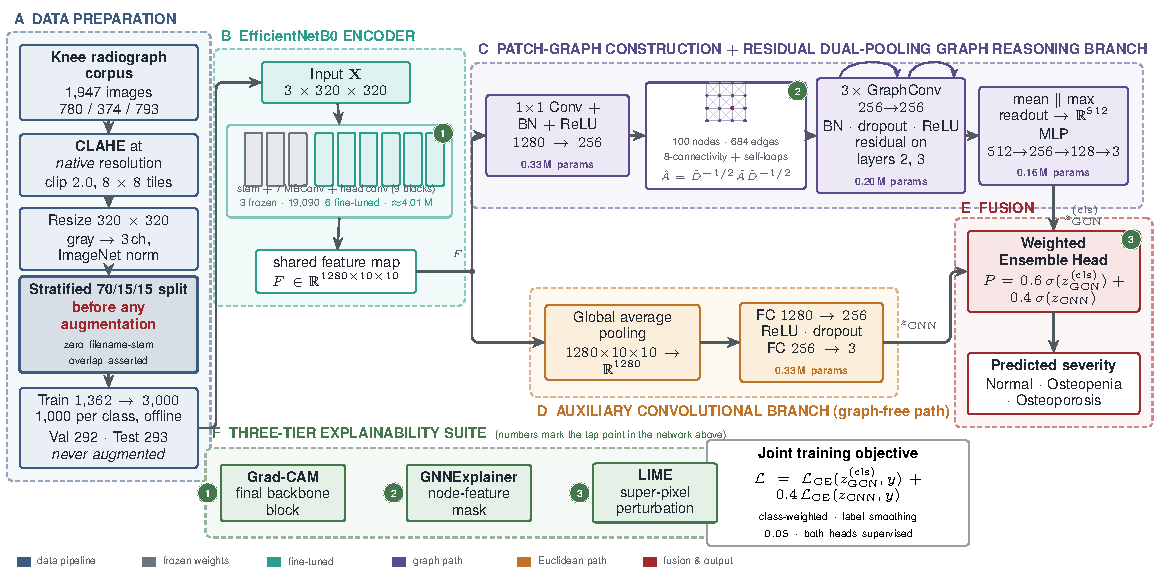
\includegraphics[width=\columnwidth]{figs_vector/fig1_pipeline_overview.pdf}
    \caption{End-to-end EfficientNet-GCN pipeline: data preparation, the EfficientNetB0 Radiographic Encoder, the Patch-Graph Construction Module feeding the Residual Dual-Pooling Graph Reasoning Branch, the parallel Auxiliary Convolutional Branch, and the Weighted Ensemble Head.}
    \label{fig:workflow_gcn}
\end{figure}

\subsection{Dataset Description}
The dataset consists of 1,947 knee radiographs collected across three diagnostic categories: Normal (780 images), Osteopenia (374 images), and Osteoporosis (793 images). The category imbalance is notable, with Osteopenia accounting for less than a fifth of the total corpus, a disparity that later shaped the augmentation strategy adopted in Section~\ref{sec:augmentation}. Images were organized by class into separate folders and read using a standard folder-labeled loader, so that class membership was inferred directly from directory structure rather than an external annotation file.

\subsection{Data Preprocessing}
Every image was first converted to grayscale, and Contrast Limited Adaptive Histogram Equalization \cite{zuiderveld1994contrast} (clip limit $2.0$, tile grid $8 \times 8$) was applied \emph{at the image's native resolution}, before any resizing. This ordering is deliberate: enhancing contrast first and resizing second preserves the fine trabecular striations that carry much of the diagnostic signal in bone-density assessment, whereas resizing first and enhancing contrast afterward would let CLAHE amplify resampling artefacts rather than genuine bone structure. No denoising filter is applied, since a low-pass step before resizing would smooth away the same trabecular texture. The contrast-enhanced image is then resized to $320 \times 320$ pixels using area interpolation when downscaling or cubic interpolation when upscaling, whichever is appropriate for the source image's native size, and the single grayscale channel is replicated across three channels to match the input expectations of an ImageNet-pretrained backbone.

The choice of enhancement parameters was not arbitrary. A preliminary bone-intensity analysis was carried out across the three classes, computing the mean and standard deviation of grayscale pixel intensity per class. This analysis surfaced a measurable, if modest, intensity gradient between Normal, Osteopenia, and Osteoporosis samples, which supported the use of a local, tile-based contrast method rather than a single global histogram stretch. At load time, images are normalized using standard ImageNet statistics (mean $0.485, 0.456, 0.406$; standard deviation $0.229, 0.224, 0.225$).

\begin{figure}[!h]
    \centering
    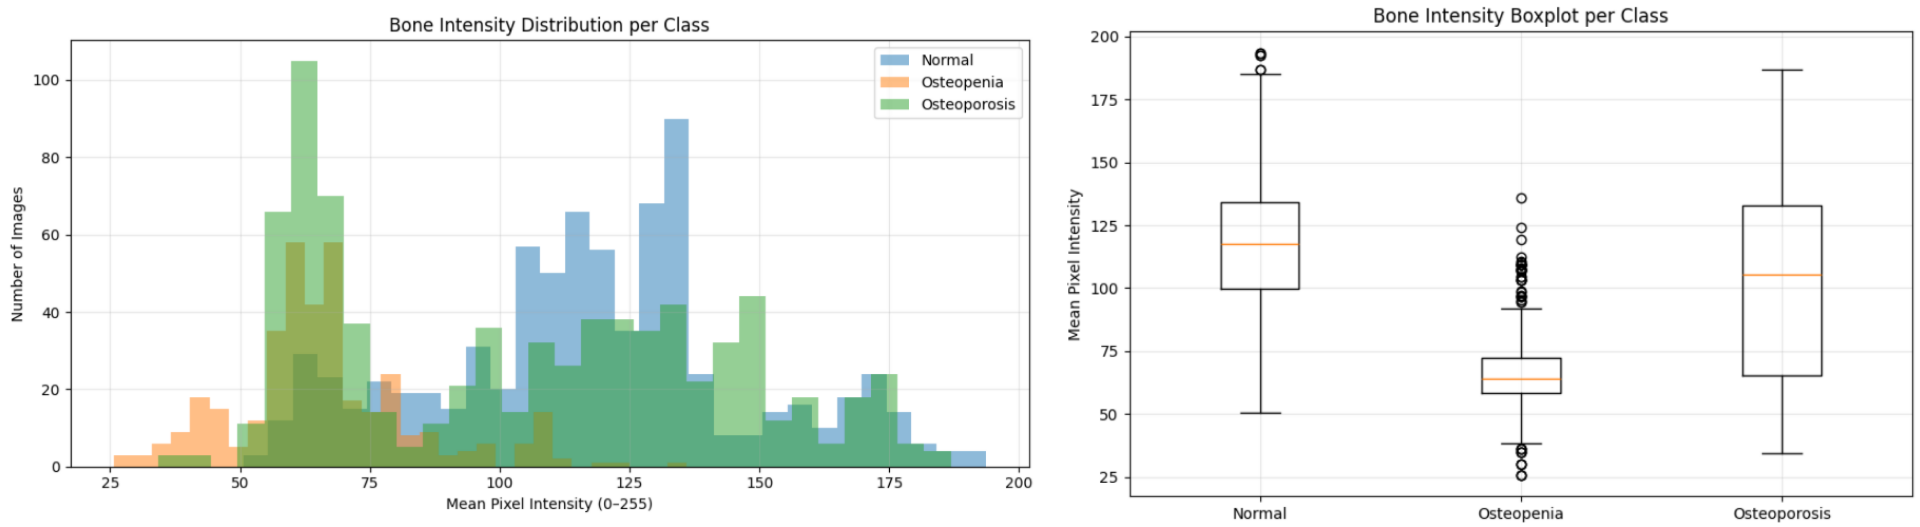
\includegraphics[width=.9\columnwidth]{bone_intensity_distribution.png}
    \caption{Bone intensity distribution per class.}
    \label{fig:intensity}
\end{figure}

\begin{figure}[!h]
    \centering
    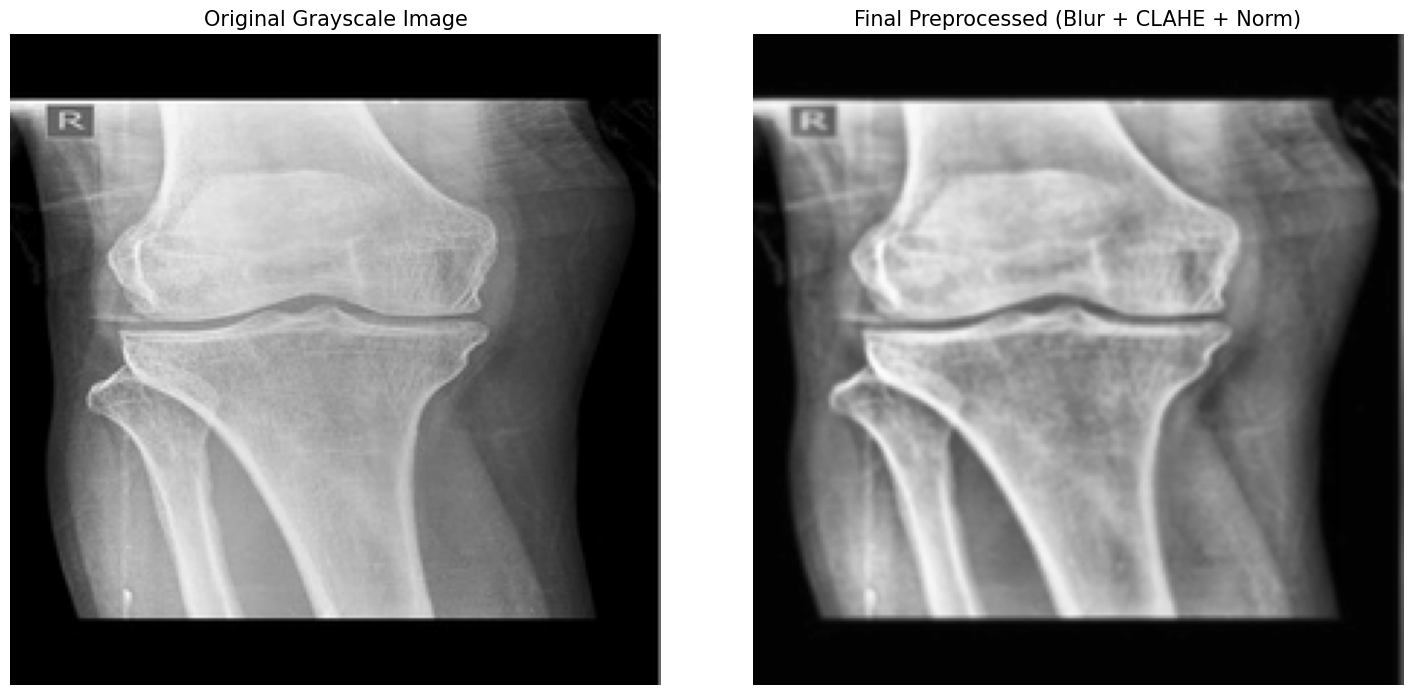
\includegraphics[width=.75\columnwidth]{preprocessed_comparison.png}
    \caption{Original versus preprocessed radiograph (CLAHE at native resolution, then resized).}
    \label{fig:preprocessed}
\end{figure}

\subsection{Dataset Split}
\label{sec:split}
Unlike a design that augments first and splits second, the split here is performed \emph{before} any augmentation, directly on the preprocessed originals: each class is divided 70/15/15 into training, validation, and test partitions (Table~\ref{tab:dataset_split}), yielding 1,362 training, 292 validation, and 293 test images overall. This ordering matters methodologically: augmenting before splitting can place near-duplicate variants of the same source radiograph in both the training and test partitions, so that reported accuracy partly reflects memorization of a specific X-ray rather than generalization to an unseen one. Splitting first guarantees that every source radiograph appears in exactly one partition; this is verified programmatically by asserting zero filename-stem overlap between the train, validation, and test directories after the split, and again after augmentation is applied. Only the training partition is subsequently rebalanced by augmentation (Section~\ref{sec:augmentation}); the validation and test partitions are left at their natural, imbalanced class distribution and are evaluated using only the deterministic preprocessing of Section~\ref{methodology}, with every metric reported as a macro average (Section~\ref{sec:metrics}) precisely because the test set is not class-balanced.

\begin{table}[!h]
\centering
\caption{Dataset Distribution: Original 70/15/15 Split, Then Training-Only Augmentation}
\label{tab:dataset_split}
\resizebox{\columnwidth}{!}{%
\begin{tabular}{|l|c|c|c|c|}
\hline
\textbf{Class} & \textbf{Train (orig.)} & \textbf{Val} & \textbf{Test} & \textbf{Train (aug.)} \\
\hline
Normal        & 546  & 117 & 117 & 1000 \\ \hline
Osteopenia    & 261  & 56  & 57  & 1000 \\ \hline
Osteoporosis  & 555  & 119 & 119 & 1000 \\ \hline
\textbf{Total} & \textbf{1362} & \textbf{292} & \textbf{293} & \textbf{3000} \\
\hline
\end{tabular}%
}
\end{table}

\subsection{Class-Balancing Augmentation}
\label{sec:augmentation}
Given the roughly two-to-one disparity between the smallest and largest classes in the training partition, training directly on the raw distribution risked biasing the classifier toward the majority classes. Rather than reweighting the loss alone, the training partition itself was rebalanced through targeted, offline augmentation, applied only after the split of Section~\ref{sec:split} and only to the training images. Every original training image is retained unchanged, and each class is then topped up with augmented variants, cycling back through the originals as needed, until it reaches 1,000 images. An Albumentations \cite{buslaev2020albumentations} pipeline supplies the augmented variants, drawing from horizontal flip ($p=0.5$), a combined affine transform with scaling in $[0.90,1.10]\times$, translation up to $6\%$ per axis, and rotation within $\pm12^{\circ}$ ($p=0.8$), brightness/contrast jitter ($p=0.5$), and additive Gaussian noise ($p=0.3$). Each transform is applied independently at its own probability rather than exactly one per image, so an augmented sample may combine several perturbations. This step brings the training partition to 1,000 images per class, 3,000 in total (Table~\ref{tab:dataset_split}); the validation and test partitions are never augmented.

A second, online augmentation stage is applied on top of this balanced training set at every training step, implemented with torchvision transforms: random resized cropping (scale $[0.85,1.0]$), random horizontal flip, random rotation up to $10^{\circ}$, brightness/contrast jitter, and random erasing ($p=0.25$) for mild occlusion robustness. Hue and saturation jitter are deliberately excluded, since the radiographs are grayscale replicated across three channels and colour perturbations would desynchronize the channels into hues that cannot occur in a real X-ray. Validation and test images instead pass through a fixed, deterministic pipeline of resizing to $320\times320$ followed by ImageNet normalization only, with no stochastic transform of any kind.

\subsection{Framework Overview and Forward Pass}
\label{sec:overview}
EfficientNet-GCN is organized around three named components, described in turn in Sections~\ref{sec:encoder}--\ref{sec:auxensemble}: a \textbf{Patch-Graph Construction Module} that channel-reduces and turns the backbone's spatial feature map into a relational patch graph, a \textbf{Residual Dual-Pooling Graph Reasoning Branch} that propagates information across that graph and reads it out, and an \textbf{Auxiliary Convolutional Branch} whose prediction is fused with the graph branch's prediction by a \textbf{Weighted Ensemble Head}. Figure~\ref{fig:workflow_gcn} summarizes the resulting end-to-end dataflow. Let $I \in \mathbb{R}^{3\times320\times320}$ denote a preprocessed input image, $E(\cdot)$ the EfficientNetB0 encoder of Section~\ref{sec:encoder}, $\mathrm{Proj}(\cdot)$ the channel-reduction step and $\mathrm{PatchGraph}(\cdot)$ the graph-construction operator of Section~\ref{sec:patchgraph}, $\mathrm{GCN}_3(\cdot)$ and $\mathrm{DualPool}(\cdot)$ the three-layer graph branch and its readout from Section~\ref{sec:gcnbranch}, and $\mathrm{MLP}_{\text{graph}}(\cdot)$ and $\mathrm{MLP}_{\text{aux}}(\cdot)$ the two branches' classification heads (Sections~\ref{sec:gcnbranch}--\ref{sec:auxensemble}). The forward pass can then be written compactly as

\begingroup
\small
\begin{equation}
\label{eq:forward}
\begin{aligned}
F &= E(I), \\
F' &= \mathrm{Proj}(F), \qquad G = \mathrm{PatchGraph}(F'), \\
z_{\text{GCN}} &= \mathrm{DualPool}\big(\mathrm{GCN}_3(G)\big), \quad z_{\text{GCN}}^{(\text{cls})} = \mathrm{MLP}_{\text{graph}}(z_{\text{GCN}}), \\
z_{\text{CNN}} &= \mathrm{MLP}_{\text{aux}}\big(\mathrm{GAP}(F)\big), \\
P_{\text{final}} &= 0.6\,\sigma\big(z_{\text{GCN}}^{(\text{cls})}\big) + 0.4\,\sigma\big(z_{\text{CNN}}\big),
\end{aligned}
\end{equation}
\endgroup

where $F \in \mathbb{R}^{10\times10\times1280}$ is the spatial feature map shared by both branches, $F' \in \mathbb{R}^{10\times10\times256}$ is its channel-reduced counterpart, $G=(V,E)$ is the 100-node patch graph of Section~\ref{sec:patchgraph}, $\sigma(\cdot)$ denotes the softmax function, and $P_{\text{final}} \in \mathbb{R}^{3}$ is the final class-probability vector reported in Section~\ref{results}. Note that the two branches deliberately consume different tensors: the graph branch reasons over the channel-reduced $F'$, while the auxiliary branch pools the full, un-reduced $F$ directly. This shared-backbone, dual-branch design lets the graph branch reason relationally over patch neighborhoods while the auxiliary branch retains a direct, graph-free path from features to logits; the two views are reconciled only at the very last step, by the ensemble of Eq.~\ref{eq:ensemble}.

\subsection{EfficientNetB0 Radiographic Encoder}
\label{sec:encoder}
The shared encoder $E(\cdot)$ is EfficientNetB0 \cite{tan2019efficientnet}, initialized from ImageNet weights. The encoder's convolutional trunk consists of a stem followed by seven MBConv stages and a final $1\times1$ head convolution, nine top-level blocks in total. Rather than freezing the entire network or fine-tuning it wholesale, only the last six of these nine blocks, the final five MBConv stages together with the head convolution, were made trainable, leaving the stem and the first two MBConv stages frozen at their ImageNet-pretrained weights; this compromise lets the network adapt its higher-level filters to radiographic texture while leaving the most generic low-level filters undisturbed. For an input of $320 \times 320$, the backbone produces the spatial feature map $F = E(I) \in \mathbb{R}^{10\times10\times1280}$, with 1,280 channels per spatial location, that feeds both downstream branches.

\subsection{Patch-Graph Construction Module}
\label{sec:patchgraph}
Before graph construction, a $1\times1$ convolution channel-reduces the shared feature map from 1,280 to 256 channels:

\begingroup
\small
\begin{equation}
\label{eq:proj}
F' = \mathrm{ReLU}\big(\mathrm{BN}(\mathrm{Conv}_{1\times1}(F))\big) \in \mathbb{R}^{10\times10\times256}.
\end{equation}
\endgroup

This projection exists purely to control the graph branch's parameter count: feeding the raw 1,280-channel features directly into a graph-convolutional layer would make that layer's weight matrix alone larger than the entire patch graph has nodes to justify, so a lightweight $1\times1$ convolution performs the same dimensionality reduction with far fewer parameters and less overfitting risk than pushing the reduction into the first graph-convolutional layer. Rather than pooling $F'$ directly, as a conventional CNN classifier would, the Patch-Graph Construction Module treats each of the one hundred spatial positions of $F'$ as a node $x_i \in \mathbb{R}^{256}$ of a graph $G=(V,E)$, $|V|=100$ (Figure~\ref{fig:architecture}, panel A). Nodes are connected to their spatial neighbors using an eight-connectivity scheme, so that each patch is linked not only to its orthogonal neighbors but also to its diagonal ones (Figure~\ref{fig:architecture}, panel B), producing 684 directed edges over the $10 \times 10$ grid. A fixed, spectral propagation rule was chosen over an attention-weighted alternative such as GAT \cite{velickovic2018graph} to keep the added parameter count small relative to the 100-node patch graph, though learned edge weighting remains a natural extension; this design choice mirrors the fixed neighborhood-graph construction used by the more general MedGNN framework \cite{ye2026medgnn}, adapted here to a regular grid whose neighborhood structure is already known rather than a learned $k$-nearest-neighbor graph. The resulting adjacency $A$ is made self-connected and symmetrically normalized before being consumed by the graph branch (Figure~\ref{fig:architecture}, panel C):

\begingroup
\small
\begin{equation}
\label{eq:selfloop}
\tilde{A} = A + I, \qquad \tilde{D} = \mathrm{diag}\Big(\textstyle\sum_{j}\tilde{A}_{ij}\Big),
\end{equation}
\endgroup

where $I$ is the identity matrix and $\tilde{D}$ is the degree matrix of the self-looped adjacency $\tilde{A}$. The node set $\{x_i\}_{i=1}^{100}$ together with the normalized adjacency $\tilde{D}^{-\frac{1}{2}}\tilde{A}\tilde{D}^{-\frac{1}{2}}$ is the graph $G$ consumed by the Residual Dual-Pooling Graph Reasoning Branch of Section~\ref{sec:gcnbranch}, and this normalized adjacency is exactly the term that appears inside Eq.~\ref{eq:gcn}.

\begin{figure}[!h]
    \centering
    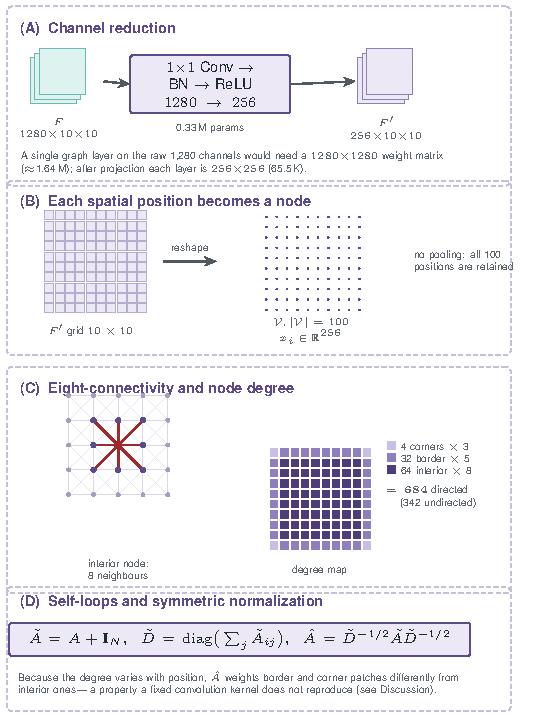
\includegraphics[width=\columnwidth]{figs_vector/fig2_patch_graph_module.pdf}
    \caption{Patch-Graph Construction Module. A $1\times1$ convolution first reduces the feature map from 1,280 to 256 channels (Eq.~\ref{eq:proj}). (A) Each of the 100 spatial positions of the reduced $10\times10$ feature map becomes one graph node. (B) An eight-connectivity scheme links every patch to its orthogonal and diagonal neighbors. (C) Self-loops are added and the adjacency is symmetrically normalized before entering the graph branch.}
    \label{fig:architecture}
\end{figure}

\subsection{Residual Dual-Pooling Graph Reasoning Branch}
\label{sec:gcnbranch}
The patch graph $G$ is processed by three stacked graph-convolutional layers, all $256 \rightarrow 256$ since the channel reduction to 256 was already performed by the Patch-Graph Construction Module (Eq.~\ref{eq:proj}), each following the standard spectral propagation rule of Kipf and Welling \cite{kipf2017semisupervised} (Eq.~\ref{eq:gcn}, Figure~\ref{fig:gcnbranch}). Each layer is followed by batch normalization, dropout, and a ReLU nonlinearity, with residual connections added around the second and third layers to ease optimization as depth increases.

\begingroup
\small
\begin{equation}
\label{eq:gcn}
H^{(l+1)} = \sigma\left(\tilde{D}^{-\frac{1}{2}}\tilde{A}\tilde{D}^{-\frac{1}{2}}H^{(l)}W^{(l)}\right)
\end{equation}
\endgroup

where $\tilde{A} = A + I$ is the patch-adjacency matrix with self-loops added (Eq.~\ref{eq:selfloop}), $\tilde{D}$ is its corresponding degree matrix, $H^{(l)}$ denotes the node features entering layer $l$, $W^{(l)}$ is the layer's learnable weight matrix, and $\sigma$ is the ReLU nonlinearity. Rather than pooling the graph with a single readout, the branch concatenates a global mean-pooling operation, capturing the overall density signal across the joint, with a global max-pooling operation, capturing the single most abnormal patch:

\begingroup
\small
\begin{equation}
\label{eq:pooling}
z_{\text{GCN}} = \big[\,\mathrm{MeanPool}\big(H^{(3)}\big) \,;\, \mathrm{MaxPool}\big(H^{(3)}\big)\,\big] \in \mathbb{R}^{512}
\end{equation}
\endgroup

This 512-dimensional graph embedding $z_{\text{GCN}}$ then passes through a two-layer fully connected head ($512 \rightarrow 256 \rightarrow 128 \rightarrow 3$) to produce the graph branch's class logits $z_{\text{GCN}}^{(\text{cls})}$.

\begin{figure}[!h]
    \centering
    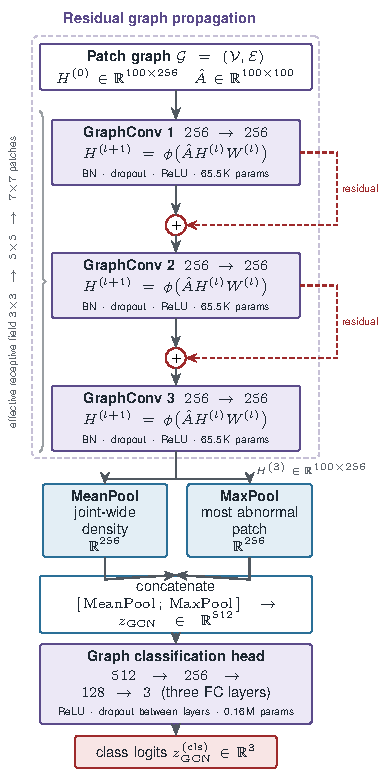
\includegraphics[width=\columnwidth]{figs_vector/fig3_gcn_branch.pdf}
    \caption{Residual Dual-Pooling Graph Reasoning Branch. Three graph-convolutional layers (Eq.~\ref{eq:gcn}) with residual connections around layers 2 and 3 produce node features $H^{(3)}$, which are read out by concatenated mean--max pooling (Eq.~\ref{eq:pooling}) and passed through the graph classification head.}
    \label{fig:gcnbranch}
\end{figure}

\subsection{Auxiliary Convolutional Branch and Weighted Ensemble Head}
\label{sec:auxensemble}
A second, considerably simpler branch operates in parallel on the same shared feature map $F$, bypassing the graph entirely (Figure~\ref{fig:auxensemble}): global average pooling followed by two fully connected layers ($1280 \rightarrow 256 \rightarrow 3$) with a ReLU activation and dropout in between, producing auxiliary logits $z_{\text{CNN}}$. This Auxiliary Convolutional Branch is trained jointly with the graph branch, and its predictions are combined with those of the GCN branch at inference time by the Weighted Ensemble Head as a weighted probability ensemble (Eq.~\ref{eq:ensemble}), with the larger weight assigned to the graph branch on the grounds that it has access to inter-patch relationships the auxiliary branch does not.

\begingroup
\small
\begin{equation}
\label{eq:ensemble}
P_{\text{final}} = 0.6 \cdot \text{softmax}(z_{\text{GCN}}^{(\text{cls})}) + 0.4 \cdot \text{softmax}(z_{\text{CNN}})
\end{equation}
\endgroup

\begin{figure}[!h]
    \centering
    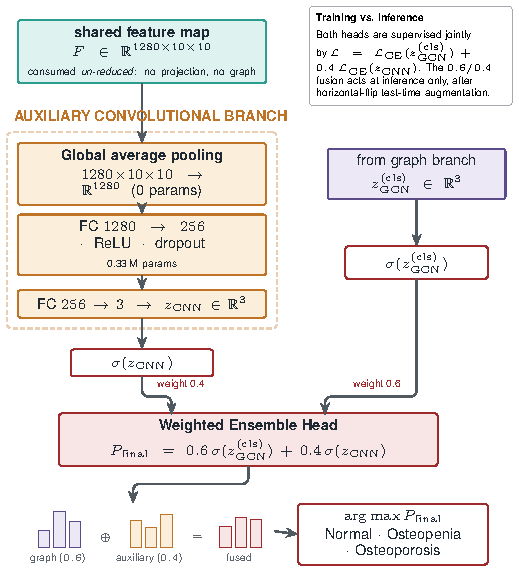
\includegraphics[width=\columnwidth]{figs_vector/fig4_auxiliary_ensemble.pdf}
    \caption{Auxiliary Convolutional Branch and Weighted Ensemble Head. The auxiliary branch pools the shared feature map directly and produces $z_{\text{CNN}}$, which is combined with the graph branch's $z_{\text{GCN}}^{(\text{cls})}$ by the 0.6/0.4 weighted probability ensemble of Eq.~\ref{eq:ensemble}.}
    \label{fig:auxensemble}
\end{figure}

\subsection{Training Configuration}
Training minimized a class-weighted cross-entropy loss with label smoothing of $0.05$, combined with a secondary cross-entropy term on the auxiliary CNN branch weighted at $0.4$ (Eq.~\ref{eq:loss}); because the training partition is already balanced by the augmentation of Section~\ref{sec:augmentation}, the inverse-frequency class weights are effectively uniform in practice. Optimization used AdamW \cite{loshchilov2019decoupled} (Eq.~\ref{eq:adamw}) with two parameter groups at differential learning rates: the unfrozen backbone layers were updated at $1 \times 10^{-4}$, while the projection layer, graph branch, and auxiliary branch were grouped together and updated more aggressively at $1 \times 10^{-3}$, both with a weight decay of $1 \times 10^{-4}$. A bare cosine schedule at this backbone learning rate destabilizes the pretrained weights in the first steps, so the learning-rate multiplier instead follows a linear warmup over the first 3 epochs, ramping from a small fraction of the base rate up to it, followed by a single cosine decay down to zero over the remaining 42 epochs, with no restarts (Eq.~\ref{eq:schedule}).

\begingroup
\small
\begin{equation}
\label{eq:loss}
\mathcal{L} = \mathcal{L}_{CE}(z_{\text{GCN}}^{(\text{cls})}, y) + 0.4\,\mathcal{L}_{CE}(z_{\text{CNN}}, y)
\end{equation}

\begin{equation}
\label{eq:adamw}
\theta_{t+1} = \theta_t - \eta_t \left( \frac{\hat{m}_t}{\sqrt{\hat{v}_t} + \epsilon} + \lambda \theta_t \right)
\end{equation}

\begin{equation}
\label{eq:schedule}
\eta_t = \eta_{\text{base}} \times
\begin{cases}
\dfrac{t+1}{T_{\text{warm}}}, & t < T_{\text{warm}} \\[4pt]
\dfrac{1}{2}\Big(1+\cos\Big(\pi\,\dfrac{t-T_{\text{warm}}}{T_{\max}-T_{\text{warm}}}\Big)\Big), & t \geq T_{\text{warm}}
\end{cases}
\end{equation}
\endgroup

with $T_{\text{warm}}=3$ warmup epochs and $T_{\max}=45$ total epochs. Gradients were clipped at a norm of $5.0$ to guard against instability introduced by the graph convolutions, training used mixed-precision (AMP) throughout except inside the graph branch, whose sparse scatter operations are run in full precision for numerical stability, and training was stopped early if validation macro-F1, rather than validation accuracy, failed to improve for ten consecutive epochs; macro-F1 is the model-selection criterion because the validation partition is naturally imbalanced (Section~\ref{sec:split}), and accuracy alone can favor a model that neglects the minority Osteopenia class. At inference, predictions were averaged across the original image and its horizontal mirror, a lightweight test-time augmentation intended to reduce sensitivity to left--right orientation.

\subsection{Experimental Setup}
\label{sec:expsetup}
All experiments were implemented in Python 3.12 using PyTorch 2.11 and PyTorch Geometric for the graph-convolutional layers, OpenCV for image preprocessing, Albumentations \cite{buslaev2020albumentations} for augmentation, and scikit-learn for evaluation metrics. Training was carried out in a Google Colab GPU runtime on a single NVIDIA Tesla T4. \textbf{[Action required: report system RAM and the exact PyTorch Geometric version if you would like these included; GPU, Python, and PyTorch versions above are taken directly from the training run's logged output.]} Table~\ref{tab:hyperparameters} summarizes the key training and inference hyperparameters used across both the graph and auxiliary branches.

\begin{table}[!t]
\centering
\caption{Training Configuration}
\label{tab:hyperparameters}
\resizebox{\columnwidth}{!}{%
\begin{tabular}{|l|c|}
\hline
\multicolumn{2}{|c|}{\textbf{Input \& Backbone}} \\ \hline
Input size & $320 \times 320$ \\ \hline
Backbone & EfficientNetB0 (last 6 of 9 blocks) \\ \hline
Projection & $1\times1$ conv, $1280\rightarrow256$ \\ \hline
Graph structure & 10$\times$10 grid, 8-connectivity \\ \hline
Graph edges & 684 \\ \hline
GCN depth & 3 layers, 256 hidden units \\ \hline
\multicolumn{2}{|c|}{\textbf{Optimization}} \\ \hline
Optimizer & AdamW (differential LR) \\ \hline
Backbone LR / Head LR & $1\times10^{-4}$ / $1\times10^{-3}$ \\ \hline
Weight decay & $1\times10^{-4}$ \\ \hline
Scheduler & Warmup (3 ep.) + cosine decay, 45 ep. \\ \hline
Loss & Cross-entropy, label smoothing 0.05 \\ \hline
Batch size & 24 \\ \hline
Mixed precision & Enabled (AMP) \\ \hline
Gradient clip norm & 5.0 \\ \hline
Checkpoint selection & Best validation macro-F1 \\ \hline
Early stopping patience & 10 epochs \\ \hline
\multicolumn{2}{|c|}{\textbf{Inference}} \\ \hline
Ensemble weight & 0.6 (GCN), 0.4 (CNN) \\ \hline
Test-time augmentation & Horizontal flip averaging \\ \hline
\end{tabular}%
}
\end{table}

\subsection{Model Evaluation Metrics}
\label{sec:metrics}
Model performance was quantified on the test set using accuracy, macro-averaged precision, recall, and F1-score, together with a full per-class classification report, confusion matrix, and one-versus-rest ROC curves summarized by a macro-averaged AUC. For each class $c$, let $TP_c$, $FP_c$, $FN_c$, and $TN_c$ denote the true positives, false positives, false negatives, and true negatives derived from the confusion matrix. Overall accuracy is defined as

\begingroup
\small
\begin{equation}
\label{eq:accuracy}
\text{Accuracy} = \frac{\sum_{c=1}^{C} TP_c}{N}
\end{equation}
\endgroup

where $N$ is the total number of test samples and $C$ is the number of classes. Macro-averaged precision and recall are given by

\begingroup
\small
\begin{equation}
\label{eq:precision}
\text{Precision}_{\text{macro}} = \frac{1}{C}\sum_{c=1}^{C}\frac{TP_c}{TP_c + FP_c}
\end{equation}

\begin{equation}
\label{eq:recall}
\text{Recall}_{\text{macro}} = \frac{1}{C}\sum_{c=1}^{C}\frac{TP_c}{TP_c + FN_c}
\end{equation}
\endgroup

and the macro-averaged F1-score, the harmonic mean of per-class precision and recall averaged across classes, is

\begingroup
\small
\begin{equation}
\label{eq:f1}
F1_{\text{macro}} = \frac{1}{C}\sum_{c=1}^{C} 2\cdot\frac{\text{Precision}_c \cdot \text{Recall}_c}{\text{Precision}_c + \text{Recall}_c}
\end{equation}
\endgroup

For the ROC analysis, each class was evaluated in a one-vs-rest scheme using the true positive rate and false positive rate,

\begingroup
\small
\begin{equation}
\label{eq:roc}
\text{TPR}_c = \frac{TP_c}{TP_c+FN_c}, \qquad \text{FPR}_c = \frac{FP_c}{FP_c+TN_c}
\end{equation}
\endgroup

The area under the resulting TPR--FPR curve was computed per class and macro-averaged across the three classes to obtain a single AUC figure.

\subsection{Explainable Artificial Intelligence (XAI) Techniques}
\label{sec:xai}
Three explainability methods were applied to the trained model, each addressing a different level of granularity. Grad-CAM \cite{gradcam} was computed over the final block of the EfficientNetB0 backbone using the graph branch's logits as the target signal, producing coarse, class-discriminative activation maps. GNNExplainer \cite{ying2019gnnexplainer} was applied directly to the trained graph head, learning an attribute-level importance mask over the one hundred graph nodes and thereby indicating which spatial patches most influenced a given prediction. Finally, LIME \cite{lime} was used to generate super-pixel-level explanations by perturbing the input image and observing the resulting change in the ensemble's output probabilities, isolating both the regions that supported a prediction and those that argued against it. Feature-attribution methods such as SHAP \cite{lundberg2017unified} were considered as a fourth complementary view but were not included in the final pipeline, since their Shapley-value estimation is substantially more expensive at the patch-graph resolution used here; extending the XAI suite to include SHAP is left for future work.

\section{Results and Discussion}\label{results}
The results section is divided into four components: training behavior, test-set performance, discriminative power and error analysis, and explainable AI outcomes.

\subsection{Training Behavior}
Training ran for a maximum of 45 epochs but was stopped early at epoch 41 after ten consecutive epochs without improvement in validation macro-F1, the model-selection criterion (Section~\ref{sec:overview}). Training accuracy rose from 63.77\% in epoch 1 to 93.30\% at the final epoch, while validation accuracy rose from 69.18\% to a peak of 87.33\% at epoch 31, the checkpoint retained for final evaluation, at which validation macro-F1 reached 85.96\%. Training and validation loss declined together over the same span (1.21 $\rightarrow$ 0.45 train; 0.98 $\rightarrow$ 0.66 val, both measured at the retained epoch 31 checkpoint), and the final train--validation accuracy gap of 8.0 points indicates mild but controlled overfitting rather than either severe underfitting or memorization. Fig.~\ref{fig:training-curves} depicts the model's training process.

\begin{figure}[!h]
    \centering
    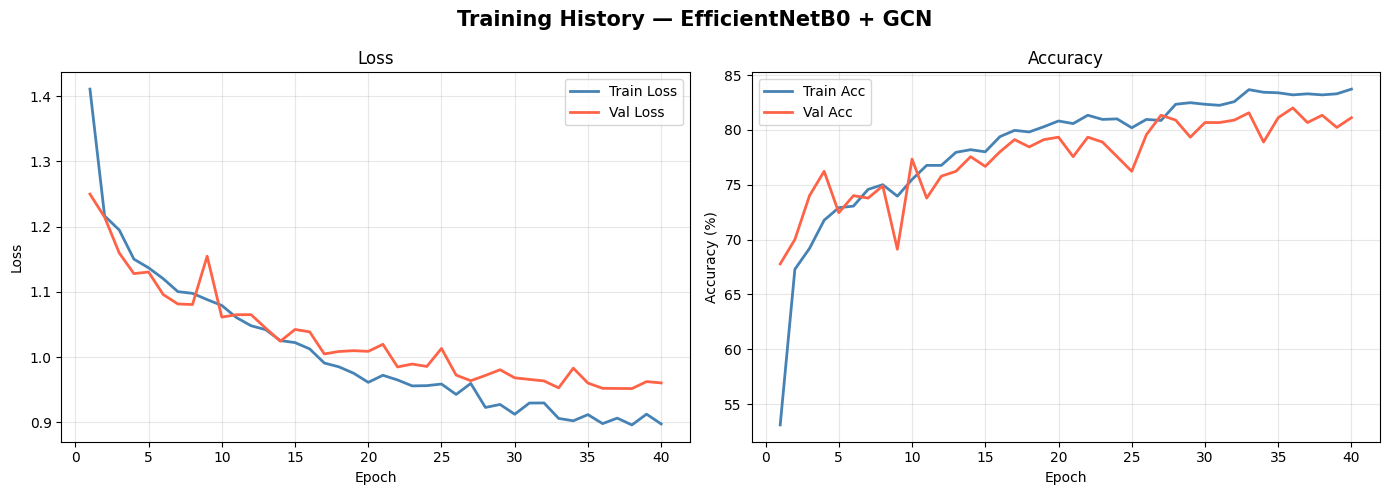
\includegraphics[width=.9\columnwidth]{gcn_training_curves.png}
    \caption{Training and validation loss/accuracy curves}
    \label{fig:training-curves}
\end{figure}

\subsection{Test Set Performance}
On the 293-image held-out test set, held at its natural, imbalanced class distribution (Section~\ref{sec:split}), the EfficientNetB0--GCN ensemble achieved an overall accuracy of 82.94\%, with macro-averaged precision, recall, and F1-score of 0.8115, 0.8227, and 0.8161 respectively (Eqs.~\ref{eq:accuracy}--\ref{eq:f1}), as detailed in Table~\ref{tab:overall_performance}. Because accuracy alone can be inflated by strong performance on the majority classes, precision, recall, and F1 are all reported as macro averages, weighting each class equally regardless of its support.

\begin{table}[!h]
\centering
\caption{Overall Test Performance}
\label{tab:overall_performance}
\begin{tabular}{|l|c|}
\hline
\textbf{Metric} & \textbf{Value} \\ \hline
Accuracy & 82.94\% \\ \hline
Precision (macro) & 0.8115 \\ \hline
Recall (macro) & 0.8227 \\ \hline
F1-score (macro) & 0.8161 \\ \hline
AUC (macro, one-vs-rest) & 0.9429 \\ \hline
\end{tabular}
\end{table}

The per-class breakdown (Table~\ref{tab:per_class_performance}) shows the model's strongest performance on the Normal class (precision 0.91, recall 0.87) and its weakest on Osteopenia (precision 0.70, recall 0.79), which is simultaneously the rarest class in the test set (57 of 293 images) and, clinically, the intermediate grade whose radiographic appearance sits closest to both of its neighbors. Osteoporosis performance falls between the two (precision 0.82, recall 0.81). This pattern, uniformly weaker precision and recall for Osteopenia rather than a strength in one and weakness in the other, is consistent with confusion concentrated at the two adjacent class boundaries (Normal--Osteopenia and Osteopenia--Osteoporosis) rather than spread evenly across all class pairs.

\begin{table}[!h]
\centering
\caption{Per-Class Performance Metrics (Test Results)}
\label{tab:per_class_performance}
\begin{tabular}{|l|c|c|c|c|}
\hline
\textbf{Class} & \textbf{Prec.} & \textbf{Rec.} & \textbf{F1} & \textbf{Support} \\ \hline
Normal        & 0.9107 & 0.8718 & 0.8908 & 117 \\ \hline
Osteopenia    & 0.7031 & 0.7895 & 0.7438 & 57 \\ \hline
Osteoporosis  & 0.8205 & 0.8067 & 0.8136 & 119 \\ \hline
\textbf{Macro avg} & \textbf{0.8115} & \textbf{0.8227} & \textbf{0.8161} & 293 \\ \hline
\end{tabular}
\end{table}

\subsection{Discriminative Power and Error Analysis}
One-vs-rest ROC analysis (Eq.~\ref{eq:roc}) yielded a macro-averaged AUC of 0.9429 (Fig.~\ref{fig:roc-curves}), indicating strong overall class separability despite the more moderate hard-label accuracy. This gap suggests the model's probability estimates rank the three classes sensibly even where the final thresholded decision is wrong -- the correct class is often placed a close second rather than the model being confidently mistaken.

\begin{figure}[!h]
    \centering
    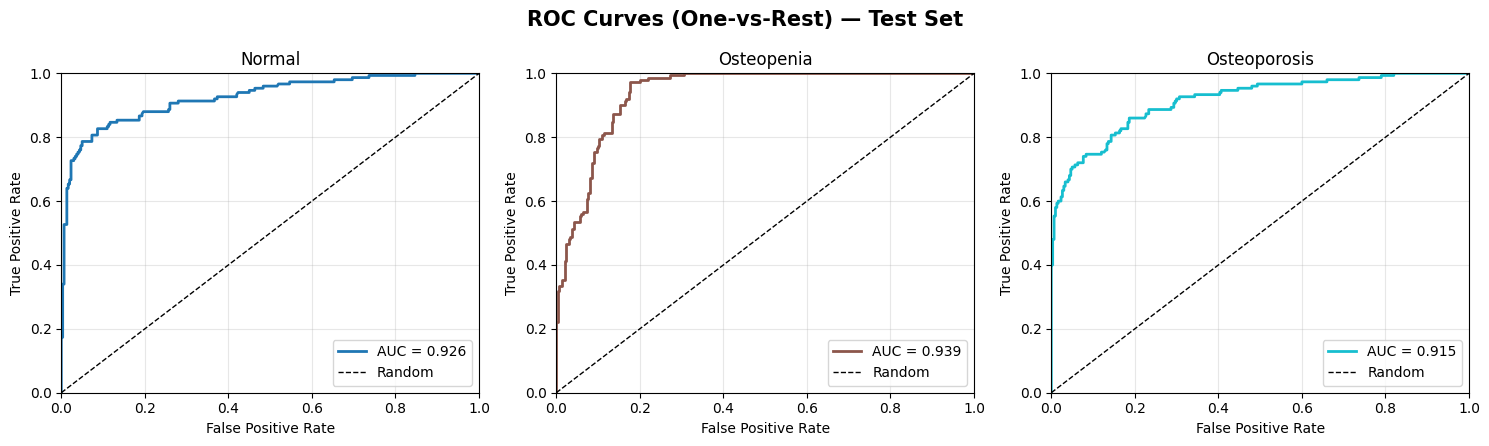
\includegraphics[width=.95\columnwidth]{gcn_roc_curves.png}
    \caption{ROC curves (one-vs-rest) per class, test set}
    \label{fig:roc-curves}
\end{figure}

Fig.~\ref{fig:confusion-matrix} details the test-set confusion matrix. Of the 293 test predictions, 19 fall on the Normal $\leftrightarrow$ Osteoporosis boundary, the costliest possible error since it corresponds to a severe case read as entirely normal or vice versa, while 31 fall on an adjacent-grade boundary (Normal--Osteopenia or Osteopenia--Osteoporosis). Errors are therefore concentrated among adjacent severity grades rather than at the clinically worst-case extremes, a reassuring property for a screening tool, even though both error counts are non-trivial on a test set of this size.

\begin{figure}[!h]
    \centering
    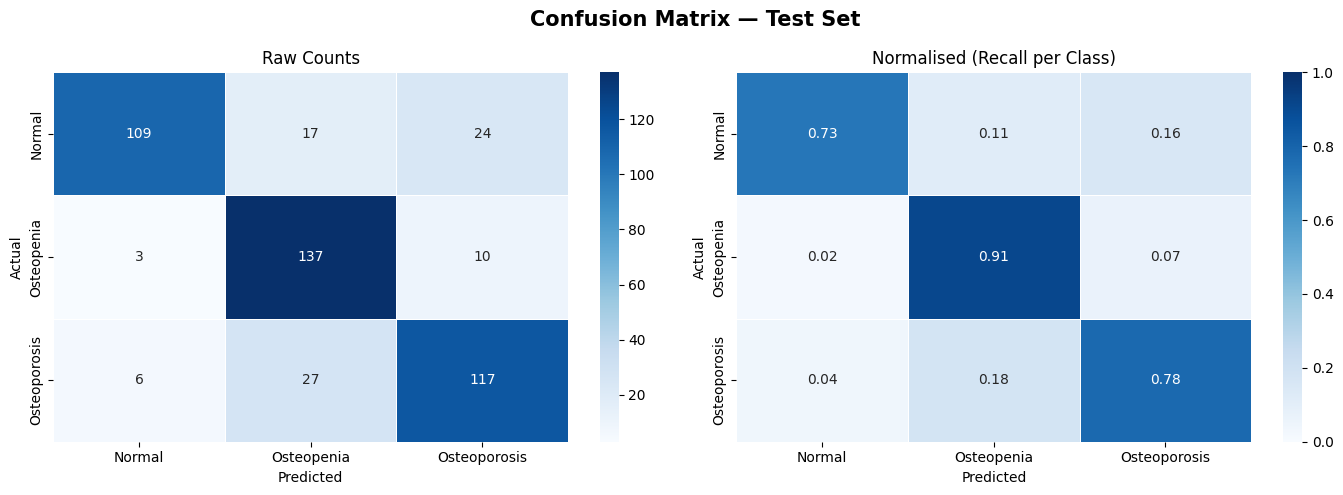
\includegraphics[width=.9\columnwidth]{gcn_confusion_matrix.png}
    \caption{Confusion matrix: raw counts and row-normalized recall, test set}
    \label{fig:confusion-matrix}
\end{figure}

\subsection{Ablation Study}
\label{sec:ablation}
To isolate the contribution of each architectural and methodological component to the 82.94\% test accuracy reported in Table~\ref{tab:overall_performance}, an ablation protocol was defined in which exactly one component of the full EfficientNetB0--GCN pipeline is removed or substituted at a time, while the data splits (Table~\ref{tab:dataset_split}), backbone, and training budget (Section~\ref{methodology}) are held fixed for every variant. Six variants were defined: (i) \textit{w/o GCN branch}, in which the patch graph and its three graph-convolutional layers are removed and the auxiliary CNN branch alone produces the final prediction, isolating the benefit of relational reasoning over patches; (ii) \textit{w/o auxiliary CNN branch}, in which the weighted ensemble of Eq.~\ref{eq:ensemble} is replaced by the GCN branch's softmax output alone, isolating the benefit of the two-branch ensemble; (iii) \textit{w/o dual pooling}, in which the concatenated mean--max graph readout is replaced by mean pooling only, isolating the benefit of retaining a max-pooled ``most abnormal patch'' signal; (iv) \textit{w/o CLAHE}, in which the contrast-enhancement step of Section~\ref{methodology} is skipped and images are resized and normalized only, isolating the benefit of native-resolution contrast enhancement; (v) \textit{w/o class-balancing augmentation}, in which the network is trained directly on the original, imbalanced 546/261/555 training distribution (Table~\ref{tab:dataset_split}) rather than the 1,000-per-class augmented set, isolating the benefit of augmentation-based rebalancing; and (vi) \textit{w/o test-time augmentation}, in which inference uses a single forward pass rather than the horizontal-flip average, isolating the benefit of TTA.

Table~\ref{tab:ablation} lists these variants alongside the full model. At the time of writing, only the full-model row reflects a completed training run, corresponding to the results already reported in Table~\ref{tab:overall_performance}; the remaining six variants are defined precisely enough to be reproduced from Section~\ref{methodology} but their retraining runs had not yet been completed at submission time, and their result columns are marked accordingly. We report the full protocol here so that the ablation can be completed and the table populated prior to camera-ready submission, and to make the intended isolation of each component transparent to reviewers in the interim.

\begin{table}[!h]
\centering
\caption{Ablation Study Protocol and Results (test set, $n=293$)}
\label{tab:ablation}
\resizebox{\columnwidth}{!}{%
\begin{tabular}{|p{3.1cm}|c|c|c|}
\hline
\textbf{Variant} & \textbf{Acc.} & \textbf{Macro F1} & \textbf{AUC} \\
\hline
Full model (proposed) & 82.94\% & 0.8161 & 0.9429 \\ \hline
(i) w/o GCN branch & \textit{pending} & \textit{pending} & \textit{pending} \\ \hline
(ii) w/o auxiliary CNN branch & \textit{pending} & \textit{pending} & \textit{pending} \\ \hline
(iii) w/o dual mean--max pooling & \textit{pending} & \textit{pending} & \textit{pending} \\ \hline
(iv) w/o CLAHE preprocessing & \textit{pending} & \textit{pending} & \textit{pending} \\ \hline
(v) w/o class-balancing augmentation & \textit{pending} & \textit{pending} & \textit{pending} \\ \hline
(vi) w/o test-time augmentation & \textit{pending} & \textit{pending} & \textit{pending} \\ \hline
\end{tabular}%
}
\end{table}

\subsection{Comparative Analysis with State-of-the-Art}
\label{sec:comparison}
Table~\ref{tab:sota_comparison} situates the proposed framework against previously published deep-learning approaches to osteoporosis and BMD assessment spanning knee, hip, spine, and dental imaging, extending the summary already given in Table~\ref{tab:osteoporosis_lit_review} with the broader-modality studies discussed in Section~\ref{Literature}.

\begin{table}[!h]
\centering
\caption{Comparison with Prior Deep Learning Approaches to Osteoporosis and BMD Assessment}
\label{tab:sota_comparison}
\resizebox{\columnwidth}{!}{%
\begin{tabular}{|p{2.1cm}|p{1.7cm}|p{0.6cm}|p{1.3cm}|p{1cm}|}
\hline
\textbf{Study} & \textbf{Modality ($n$)} & \textbf{Cls.} & \textbf{Reported Result} & \textbf{Params (M)} \\
\hline
Sukegawa et al.~\cite{sukegawa2022identification} (2022) & Panoramic dental (778) & 2 & 84.50\% acc. & N/R \\ \hline
Wani \& Arora~\cite{wani2023osteoporosis} (2023) & Knee X-ray (381) & 3 & 91.10\% acc. & N/R \\ \hline
Feng et al.~\cite{Feng2024} (2024) & Hip X-ray (139) & 3 & 74.00\% acc. & N/R \\ \hline
Naguib et al.~\cite{Naguib2024} (2024) & Knee X-ray (611) & 3 & 83.74\% acc. & N/R \\ \hline
Sarhan et al.~\cite{Sarhan2024} (2024) & Knee X-ray (1{,}947) & 3 & 97.50\% acc. & N/R \\ \hline
Chen et al.~\cite{Chen2024} (2024) & Hip X-ray (3{,}460) & Multi + T-score & 97.20\% acc. & N/R \\ \hline
Hsieh et al.~\cite{hsieh2021automated} (2021) & Pelvis/lumbar X-ray ($>$5{,}000) & 2 & 91.7\% / 86.2\% acc. & N/R \\ \hline
Zhang et al.~\cite{zhang2020deep} (2020) & Lumbar X-ray (2{,}510) & 2 & AUC 0.77--0.81 & N/R \\ \hline
Galbusera et al.~\cite{galbusera2024estimating} (2024) & Lumbar MRI/X-ray (429) & 2 & AUC 0.80--0.82 & N/R \\ \hline
Park et al.~\cite{park2024automated} (2024) & CT (422) & 2 & AUC 0.77--0.79 & N/R \\ \hline
\textbf{Proposed (this work)} & Knee X-ray (1{,}947; train balanced to 3{,}000) & \textbf{3} & \textbf{82.94\% acc., AUC 0.9429} & \textbf{5.03} \\ \hline
\end{tabular}%
}
\end{table}

Most reviewed studies do not report parameter counts alongside accuracy, which is itself a transparency gap noted in Section~\ref{gaps}; the corresponding cells are marked \emph{N/R} (not reported) rather than estimated. The proposed model's own parameter count, 5,027,970 (5.03M) in total, of which 5,008,880 (99.6\%) are trainable under the partial fine-tuning scheme of Section~\ref{sec:encoder}, was obtained directly from the trained model (\texttt{sum(p.numel() for p in model.parameters())}) rather than estimated, and breaks down as 4.01M in the EfficientNetB0 backbone, 0.33M in the projection layer, 0.36M in the graph branch, and 0.33M in the auxiliary branch.

Raw accuracy figures in Table~\ref{tab:sota_comparison} should be read with caution rather than ranked directly: the compared studies differ in class count, imaging modality, dataset size, and label source, all of which affect the difficulty of the underlying decision problem. Binary osteoporosis-vs-not formulations enjoy a structurally easier decision boundary than the three-class Normal/Osteopenia/Osteoporosis triage attempted here, which accounts for part of the gap against Sarhan et al.\ \cite{Sarhan2024} and Chen et al.\ \cite{Chen2024}, both of which report figures above 97\% on coarser class splits with larger, single-institution training sets. Within the stricter three-class knee-radiograph setting most comparable to this study, the proposed framework's 82.94\% accuracy is competitive with Naguib et al.'s \cite{Naguib2024} 83.74\% obtained on a smaller 611-image dataset, and clearly exceeds Feng et al.'s \cite{Feng2024} 74.00\% obtained on an even smaller hip cohort. Beyond raw accuracy, the framework's principal contribution relative to this literature is architectural rather than purely numerical: to our knowledge it is among the first to combine explicit graph-based relational reasoning over patch-level features with a dual CNN/GCN ensemble for osteoporosis severity classification, and it is the only entry in Table~\ref{tab:sota_comparison} to jointly report three complementary explainability views (Grad-CAM, GNNExplainer, and LIME) rather than relying on a single coarse saliency method or omitting explainability altogether.

\subsection{Explainable AI Results}
Three complementary explainability methods were applied to the trained model. Grad-CAM, computed on the final EfficientNetB0 block, consistently localized activations over cortical and medullary bone regions for correctly classified Osteopenia and Osteoporosis cases rather than diffusing over background or soft tissue (Fig.~\ref{fig:gradcam}). GNNExplainer, applied to the graph head, identified a small, spatially contiguous cluster of patch-graph nodes as the dominant contributors to each prediction (Fig.~\ref{fig:gnnexplainer}), supporting the premise that relational reasoning across neighboring bone regions carries signal beyond any single patch in isolation. LIME's super-pixel explanations (Fig.~\ref{fig:lime}) were broadly consistent with the Grad-CAM findings, with positive regions concentrating over trabecular and cortical structures for both Osteopenia and Osteoporosis predictions.

\begin{figure}[!h]
    \centering
    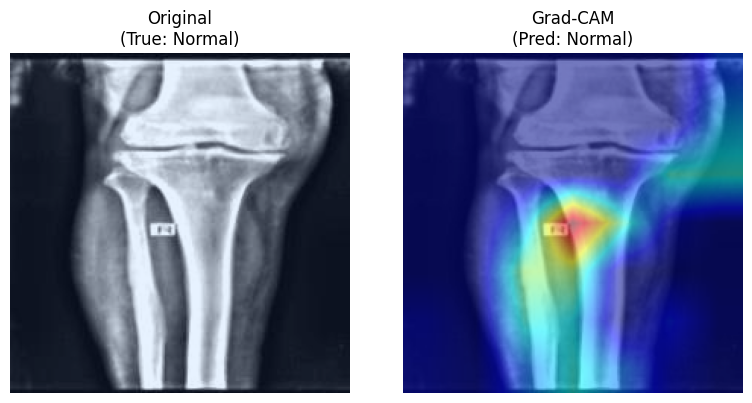
\includegraphics[width=.85\columnwidth]{gradcam_examples.png}
    \caption{Explainable AI: Grad-CAM activation overlays on representative test samples}
    \label{fig:gradcam}
\end{figure}

\begin{figure}[!h]
    \centering
    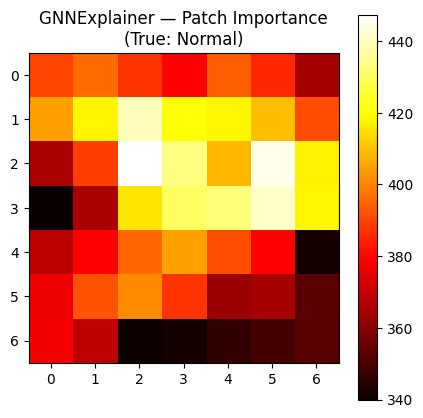
\includegraphics[width=.85\columnwidth]{gnn_explainer_overlay.png}
    \caption{GNNExplainer patch-importance heatmap and overlay on original radiograph}
    \label{fig:gnnexplainer}
\end{figure}

\begin{figure}[!h]
    \centering
    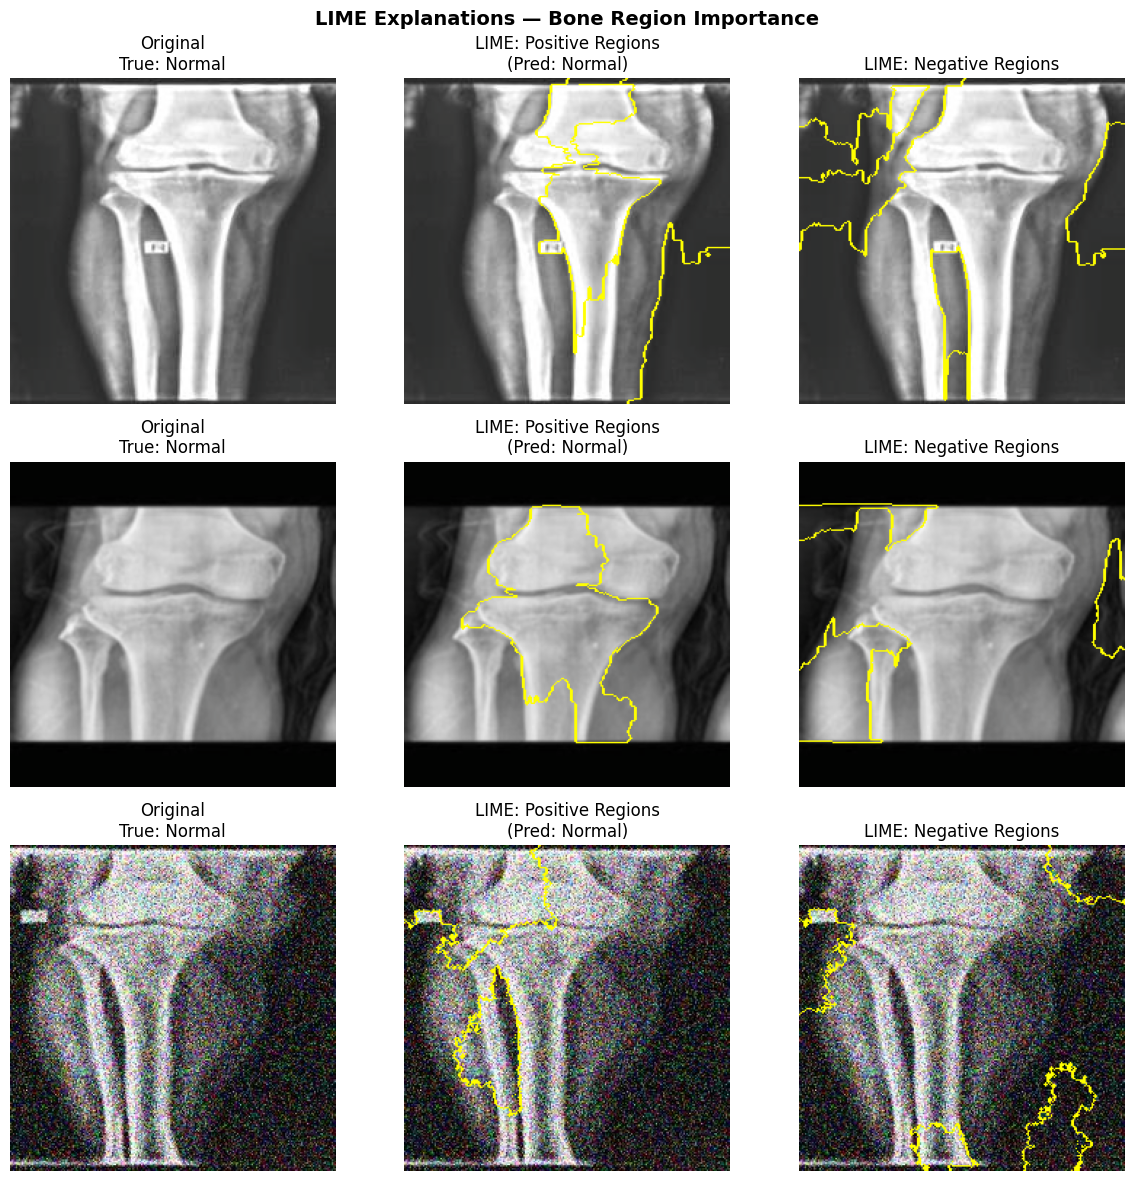
\includegraphics[width=.9\columnwidth]{lime_bone_explanations.png}
    \caption{LIME positive and negative super-pixel explanations across three test samples}
    \label{fig:lime}
\end{figure}


\section{Limitations}
\label{sec:limitations}
This study has four main limitations. First, and most importantly for interpreting Table~\ref{tab:ablation}, six of the seven ablation variants remain unrun: the protocol isolating the graph branch, auxiliary branch, dual pooling, CLAHE preprocessing, class-balancing augmentation, and test-time augmentation is fully specified in Section~\ref{sec:ablation}, but only the full model's row currently reflects a completed training run. Second, consistent with Gap 5 identified in Section~\ref{gaps}, the framework has been evaluated on a single institutional dataset \cite{gobara2024multiclass} and has not yet been tested on independent, multi-center clinical data, so its generalization across scanners and acquisition protocols remains unverified. Third, because the validation and test partitions are deliberately left at their natural, imbalanced distribution to avoid the leakage that a balance-then-split design would introduce (Section~\ref{sec:split}), the Osteopenia class is evaluated on only 57 test images, and its reported precision and recall (Table~\ref{tab:per_class_performance}) are consequently the least statistically stable of the three classes. Fourth, radiographic severity labels were taken as provided by the source dataset rather than confirmed against DEXA-based T-scores, so some label noise at the class boundaries the model confuses most often (Section~\ref{results}) cannot be ruled out.

\section{Future Work}
\label{sec:futurework}
Completing the ablation runs defined in Section~\ref{sec:ablation} and populating Table~\ref{tab:ablation} is the most immediate item of future work, since it is the most direct way to confirm which named component contributes most to the 82.94\% test accuracy. Beyond this, priority should be given to external, multi-center validation to establish generalization across imaging sources; to collecting more Osteopenia cases so that this minority class can be evaluated with the same statistical confidence as the other two; to replacing the fixed eight-connectivity patch adjacency with a learned edge-weighting scheme, following the attention-based GAT formulation \cite{velickovic2018graph} or the $k$-nearest-neighbor construction of MedGNN \cite{ye2026medgnn}; and to extending the framework toward finer-grained severity grading and lighter-weight deployment for point-of-care screening.

\section{Conclusion} \label{conclusion}
This paper presents EfficientNet-GCN, a hybrid framework for osteoporosis severity classification from knee X-ray images, built around three named components: a Patch-Graph Construction Module, a Residual Dual-Pooling Graph Reasoning Branch, and an Auxiliary Convolutional Branch fused through a Weighted Ensemble Head. An ImageNet-pretrained EfficientNetB0 encoder extracts discriminative spatial features; the Patch-Graph Construction Module channel-reduces and reformulates these features into a 100-node, eight-connected graph; and the Residual Dual-Pooling Graph Reasoning Branch propagates relational context across that graph, treating anatomically adjacent regions of the knee joint as connected nodes rather than isolated units. The Auxiliary Convolutional Branch is combined with the graph branch through a probability ensemble to stabilize predictions and reduce variance. The dataset is split into training, validation, and test partitions before any augmentation is applied, and only the training partition is subsequently rebalanced, so that the validation and test partitions retain their natural class distribution and the 82.94\% test accuracy and macro-averaged AUC of 0.9429 the model reaches reflect performance on images the model has not seen in any form. The model grounds its predictions in clinically meaningful bone regions rather than incidental artifacts, as confirmed by Grad-CAM, GNNExplainer, and LIME (Section~\ref{sec:xai}). Against prior deep-learning approaches to osteoporosis and BMD assessment (Section~\ref{sec:comparison}), the framework is competitive within the stricter three-class knee-radiograph setting and is, to our knowledge, the only compared method to combine explicit graph-based relational reasoning with three complementary levels of explainability, while also being one of the few to report its own parameter count (5.03M) alongside accuracy. Section~\ref{sec:limitations} and Section~\ref{sec:futurework} detail, respectively, the specific gaps that remain and the concrete steps planned to close them, foremost among them completing the ablation study and pursuing external, multi-center validation.

\section*{Data Availability}
The knee radiograph dataset used in this study, the Multi-Class Knee Osteoporosis X-Ray Dataset, is publicly available on Kaggle \cite{gobara2024multiclass} at \url{https://www.kaggle.com/datasets/mohamedgobara/multi-class-knee-osteoporosis-x-ray-dataset}. Source code is not publicly available. \textbf{[Action required: if a GitHub (or other) repository for this project exists or is planned, replace the preceding sentence with its link, the programming language, and the framework/version used, per the assignment's code-availability requirement.]}


\bibliographystyle{IEEEtran}
\bibliography{ref}
\end{document}
